\section{The general minimum makespan parallel motion planning problem on a grid is NP-hard}\label{chapter:main_proof}

% PRELIMINARIES
\subsection{Theorem-specific preliminaries}

A (deterministic) \emph{Turing Machine} (TM) is a mathematically modeled machine capable of general purpose computations operating on a tape of symbols. 
It is generally considered to be equivalent in capabilities to most mathematical definitions of computation. 
See \cite{aw/HopcroftU79} for a formal definition.

A \emph{decision problem} is a computational problem asking a yes/no question based on some input.

There are different \emph{classes} of decision problems in terms of computational complexity. 
The \emph{P}-class of problems is defined as the set of decision problems solvable by a TM in \emph{polynomial time}, i.e.\ in \(O(n^k)\) time on the size of the input \emph{n} and some constant \emph{k}.

The \emph{NP}-class of problems is defined as the set of decision problems that are \emph{verifiable} by a TM in polynomial time. 
Actually finding a solution to an NP-problem might take considerably longer. 
It remains an important open question whether P is or is not equal to NP, but many believe P is a proper subset of NP.

A transformation of a problem \(B\) into another problem \(A\) such that a solution to \(A\) solves \(B\) is called a \emph{reduction} and is commonly denoted \(B \leq A\). 
If the reduction can be done in polynomial time, we write \(B \leq_p A\).

\begin{definition}\label{def:np_complete}
	A decision problem \emph{A} is \emph{NP-complete} (\(A \in \text{NPC}\)) if and only if \emph{A} is in NP and there exists a polynomial time reduction from every problem in NP to \emph{A}:
	\begin{align*}
		A \in \text{NPC} \Leftrightarrow \parens{A \in \NP} \land \parens{B \leq_p A, \; \forall B \in \NP}
	\end{align*}
	NP-complete is essentially the hardest class of problems that can be verified in polynomial time. 
\end{definition}

\begin{remark}\label{rem:p_np_disjoint}
	If \(\pclass \neq \NP\) holds, the classes of P and NP-complete problems are disjoint. Otherwise \emph{all} problems in NP would be polynomially reducible to problems solvable in polynomial time, thus also solvable themselves in polynomial time. This would imply P = NP:
	\begin{align*}
		& \pclass \cap \text{NPC} \neq \emptyset \\
		\Rightarrow \; & \exists A \in \pclass : B \leq_p A, \; \forall B \in \NP \\
		\Rightarrow \; & B \in \pclass, \; \forall B \in \NP \\
		\Rightarrow \; & \pclass = \NP
	\end{align*}
\end{remark}

\begin{definition}\label{def:np_hard}
	A problem \emph{H} is classified as \emph{NP-hard} if there exists a polynomial time reduction \(A \leq_p H, \; \forall A \in \NP\). 
	Note that \(H\) begin NP-hard does \emph{not} imply \(H \in \NP\). 
	Though if \(H\) can be proven to belong to NP, i.e. be verifiable in polynomial time, \(H\) will then by definition be NP-complete.
\end{definition}

\begin{remark}\label{rem:p_np_hard_disjoint}
	The same construction as in \cref{rem:p_np_disjoint} works here too, P and NP-hard problems are disjoint, assuming \(\pclass \neq \NP\).
\end{remark}

\begin{remark}\label{note:npc_proving}
	Let \(A\) be some known NP-complete problem. 
	If there is a polynomial time reduction from \(A\) to some other problem \(B\): \(A \leq_p B\), we know that \(B\) is NP-hard. 
	Further proving that \(B\) is NP-complete would require \emph{either} a polynomial reduction from \(B\) to \(A\): \(B \leq_p A\) \emph{or}, possibly easier, proving that \(B\) is in NP, i.e. proving that \(B\) is deterministically verifiable in polynomial time.
\end{remark}

Let a \emph{boolean expression} be composed of boolean variables \(b \in \set{\true,\, \false}\), negations (\texttt{not } \(\neg\)), conjunctions (\texttt{and} \(\land\)), disjunctions (\texttt{or} \(\lor\)) and parentheses.

The following is an example of a boolean expression:
\begin{align}\label{ex:boolean_xor}
	\parens{b_1 \lor b_2} \land \neg \parens{b_1 \land b_2}
\end{align}

Let a \emph{literal} be a variable \(b\) (a positive literal) or the negation of a variable \(\neg b\) (a negative literal). 
A (disjunctive) \emph{clause} is then defined as a disjunction of literals \(C = \parens{l_1 \lor l_2 \lor \dots \lor l_k}, \ l_i \in \set{b_j,\ \neg b_j}\). 

Let a boolean expression be in \emph{Conjunctive Normal Form} (CNF) if and only if it is composed only of conjunctions of disjunctive clauses. 
The previous example in \cref{ex:boolean_xor} is \emph{not} in CNF, as negation of a clause is not allowed, and the second parenthesis is a conjunction, not a disjunction.

\begin{remark}
	It is always possible, but non-trivial, to transform an arbitrary boolean expression into CNF \cite{aw/RN2020}.
	The expression in \cref{ex:boolean_xor} can be stated in CNF as follows:
	\begin{align}\label{ex:cnf_xor}
		\parens{b_1 \lor b_2} \land \parens{\neg b_1 \lor \neg b_2}
	\end{align}
\end{remark}

Let \(\varphi\) be a boolean expression in Conjunctive Normal Form. 
The boolean satisfiability problem, abbreviated \emph{SAT}, is a decision problems asking whether \(\varphi\) can be evaluated to \true\ for some state of its variables \(\set{b_1, b_2, \dots, b_n} \in \set{\true, \false}^{n}\). 
It is trivial to verify if a solution is correct or not: a boolean expression can be evaluated well within polynomial time, thus SAT has to be in NP. 
On the other hand, there are an exponential amount of states of the input variables: \(2^n\) states for the \(n\) input variables to be exact. 
It has been proven that SAT is NP-complete \cite{coco/Karp72}, and a sub-exponential algorithm for solving a general SAT problem would be groundbreaking. 

The corresponding SAT problem to \cref{ex:cnf_xor} would ask whether \(\varphi\) is satisfiable. 
This particular expression is satisfiable, as when \(\coord{b_1}{b_2} = (\true, \false)\) or \(\coord{b_1}{b_2} = \coord{\false}{\true}\) the expression evaluates to \true, coincidentally equivalent to an \texttt{xor}\ expression.

\begin{definition}
	\emph{3SAT} is a sub-problem of SAT where each input instance has exactly 3 literals in each clause. 
	3SAT is also known to be NP-complete.
\end{definition}

\begin{definition}
	A \emph{Monotone 3SAT} is defined as a further restricted version of 3SAT, where each clause of the expression has all-positive or all-negative literals.
\end{definition}

% Boolean expressions are constructed from positive and negative literals (\(x} and \(\neg x} respectively), conjunctions (AND \(\land}), disjunctions (OR \(\lor}) and parentheses. An example SAT problem would ask whether \(}









% MAIN THEOREM
\subsection{The theorem}

Let a decision problem formulation of minimum makespan motion planning be as follows: Given a problem instance \(I \coloneqq \parens{G,\ \conf{s},\ \conf{t}}\), determine if there exists a schedule with makespan at most \emph{M} that can transform \(\conf{s} \rightarrow \conf{t}\).

\begin{lemma}\label{lemma:np}
	The decision problem formulation of a minimum makespan motion planning problem on a grid is in NP.
\end{lemma}

\begin{proof}
	It is easy to show that the decision problem is in NP; to verify a found solution, one has to check three things:
	\begin{enumerate}
		\item Every transformation step of a schedule should be valid according to \cref{req:limited_movement} and \cref{req:no_swaps}.\label{checks:transformations}
		\item After the last step of execution, the configuration should equal that of \(\conf{t}\).\label{checks:target_acquired}
		\item There should be at most \(M\) transformation steps.\label{checks:makespan}
	\end{enumerate}
	\cref{req:limited_movement} can be checked in linear time with respect to the robots for each timestep. 
	\cref{req:no_swaps} will need to be checked for each single-robot move, which is bounded by the number of robots for each timestep. 
	Thus \cref{checks:transformations} can be checked in \(\mathcal{O}(M \cdot N)\) time, where \(M\) is the makespan and \(N\) is the number of robots.
	\cref{checks:target_acquired} can be done linearly with respect to the number of robots, as checking the positions for every robot is sufficient (configurations are assumed to be valid, and that \(\iconf{}{r}\) would raise an error if the mapped position would not be deterministically defined).
	Trivially \cref{checks:makespan} can be done in \(\mathcal{O}(M)\). 
	% \fda{be careful, because items 1 and 2 need also to be repeated for at most \(M\) times: it needs to be added in the final running time}

	A solution is thus verifiable in \(\mathcal{O}(M \cdot N)\), which implies the problem is in NP by definition.
\end{proof}

\begin{theorem}\label{thm:npc}
	The decision problem formulation of a minimum makespan motion planning problem on a grid is NP-complete.
\end{theorem}

\begin{proof}
	The following proof, heavily based on the proof by \cite{siamcomp/DemaineFKMS19} is done by a polynomial reduction from \emph{Monotone 3SAT} to a decision formulation of a coordinated multi-robot motion planning problem. 
	As Monotone 3SAT is known to be NP-complete, a polynomial reduction implies the reduced problem is NP-hard. 
	Together with \cref{lemma:np}, this implies the problem is also NP-complete. 






% REDUCTION
	\subsubsection*{The reduction} 
	Let \(\varphi\) be some boolean expression corresponding to some Monotone 3SAT problem. 
	The idea is to construct a workspace with robots having start and target configurations \(\conf{s}\) and \(\conf{t}\) respectively such that a critical makespan \emph{M} is achievable if and only if the original expression \(\varphi\) is satisfiable, otherwise requiring \(M + 1\) transformation steps at a minimum to transform \(\conf{s} \rightarrow \conf{t}\). 
	Follow along the construction by observing \cref{fig:full_reduction}: a one-to-one sketch of the simplest possible example. 





% FIGURE
\begin{figure}[h]
	\centering
	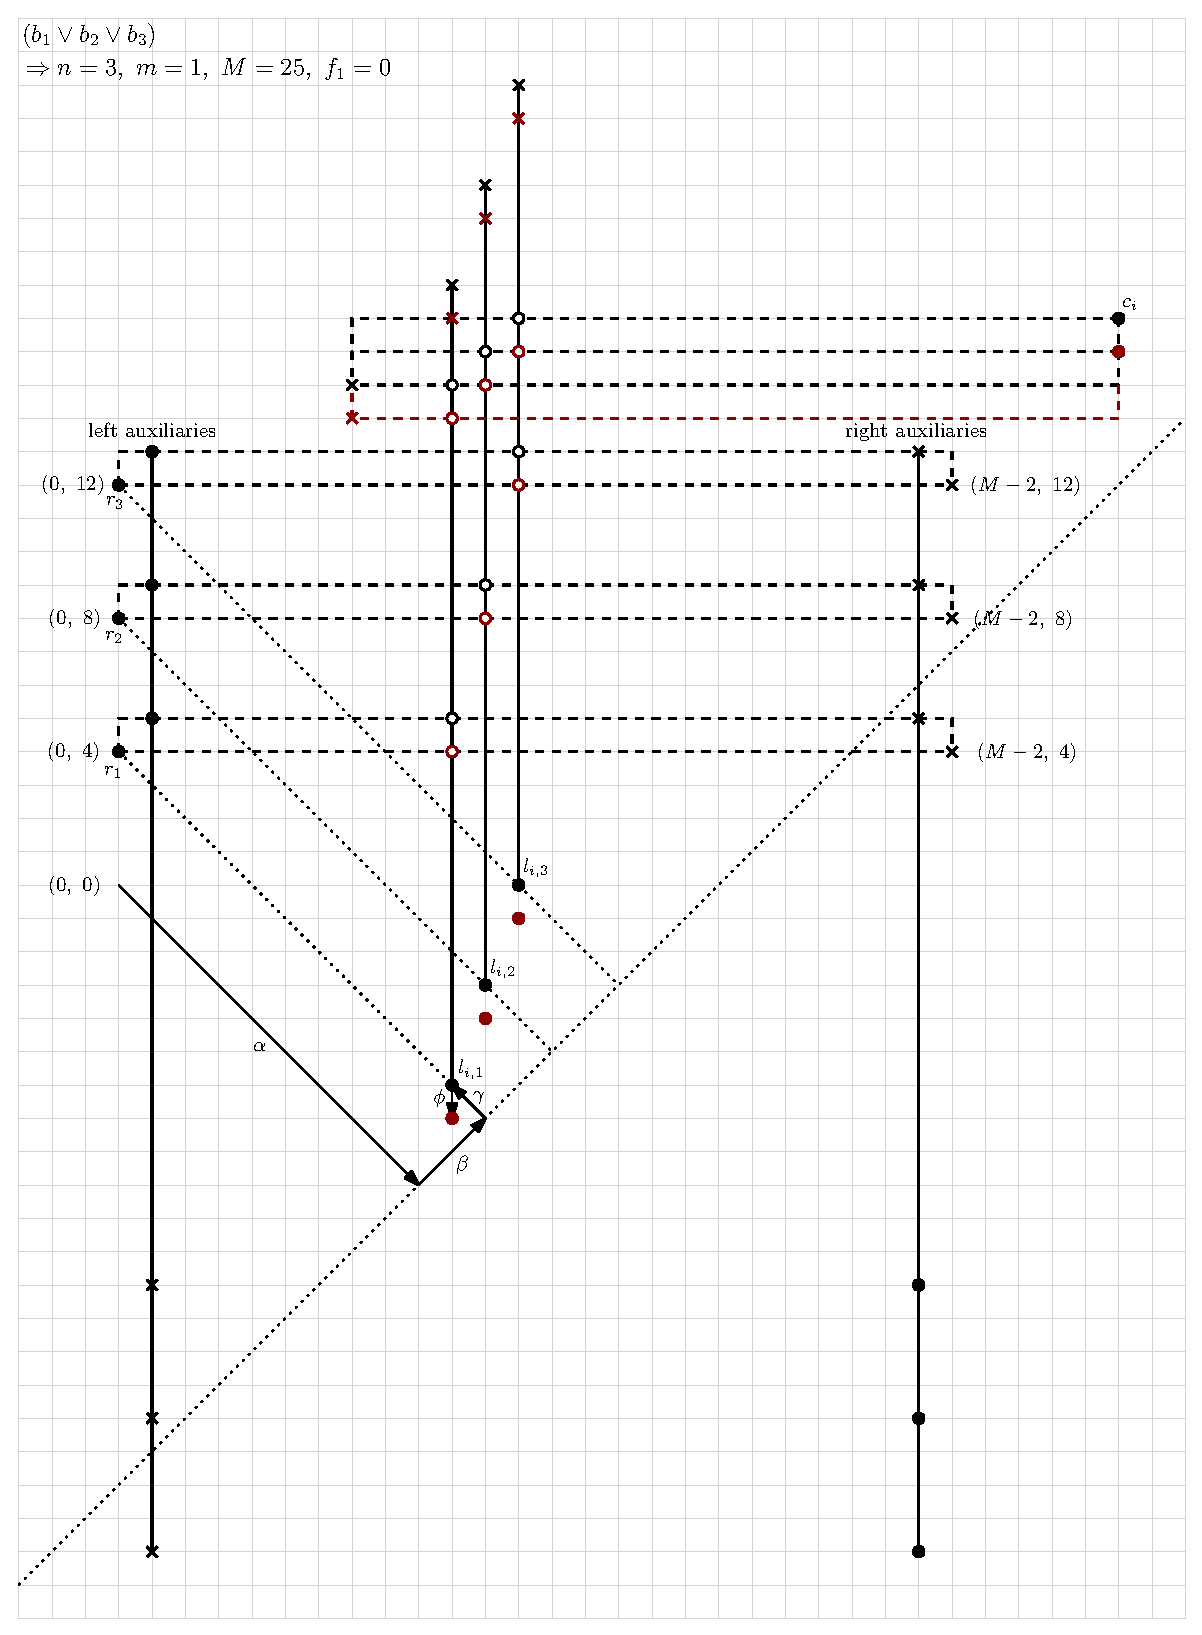
\includegraphics[height=15cm]{ipe/np_reduction.eps}
	\caption{
		A minimal Monotone 3CNF formula \(\varphi = \parens{b_1 \lor b_2 \lor b_3}\) reduced to a robot motion planning problem. 
		The dark red graphics show how the robots would be offset if the clause \(c_i\) was all-negative instead of the current all-positive. 
		Disks represent robots while crosses represent their target positions. 
		The circles highlight the variable-literal couplings and literal-clause couplings: a mismatched assignment of \(b_{j_k}\) w.r.t. \(l_{i,k}\) cascades into \(l_{i,k}\) blocking the path of \(c_i\).
	}\label{fig:full_reduction}
\end{figure}





	% Let our target makespan \emph{M} be fixed at the end of the construction, so that a schedule with makespan \emph{M} is achievable if and only if the original expression \(\varphi\) is satisfiable, otherwise a schedule with makespan \(M + 1\). 

	The formula \(\varphi\) is composed of \(n\) boolean variables \(\set{b_1, b_2, \dots, b_n}\) and \(m\) clauses \(\set{C_1, C_2, \dots, C_m}\) with three literals each. 
	Let our variables be represented by \(n\) \emph{variable robots} \(\set{r_1, r_2, \dots, r_n}\). 
	These will be able to `choose' one of two paths independently of one another, representing \true\ and \false\ assignments to them. 
	The variable robots are coupled in a many-to-many mapping to the clauses by \(3m\) \emph{literal robots}: \(\set{l_{i,k} \mid i \in \set{1, \dots, m},\ k \in \set{1, 2, 3}}\). 
	They are positioned so that they pass by their corresponding variable robot, and have to wait if the variable assignment is mismatched with the literal. 
	There are finally \(m\) \emph{clause robots} to ensure that at least one literal per simulated clause evaluates to \true. 
	This is accomplished by the clause robot having a clear path to its target only if at least one corresponding literal robot has not needed to wait for its variable robot. 
	The workspace is constructed so that any robot deviating from its constrained path results in a schedule with makespan \(> M\).

	% is made so a makespan \(M\) is only achievable if every clause robot is not blocked by a literal robot on its path, and all robots are constrained by the makespan to behave like .

	There are some details to deal with: the variable robots have to be constrained to be able to take exactly two distinct paths, while the literal robots have to be positioned to get the correct timing with its corresponding variable robot and clause robot simultaneously.

	Let the variable robot \(r_j\) have a start position at \(\coord{0}{4j}\) and target position at \(\coord{M - 2}{4j}\). 
	Notice there is exactly two timesteps to spare with respect to the critical makespan \(M\). 
	Let there be a \emph{left auxiliary robot} and a \emph{right auxiliary robot} for each variable robot. 
	The left auxiliary starts at \(\coord{1}{4j + 1}\) and travels down to \(\coord{1}{4j + 1 - M}\), while the right auxiliary starts at \(\coord{M - 3}{4j + 1 - M}\), and moves up to \(\coord{M - 3}{4j + 1}\). 
	The auxiliaries have to move exactly \(M\) steps, and thus cannot wait for \(r_j\). 
	Thus \(r_j\) is blocked from moving right at timestep 0 by the left auxiliary, and required to pass \(x = M - 3\) before timestep \(M\) to avoid blocking the right auxiliary. 
	As a result, \(r_j\) has exactly two options: wait at timesteps \(0\) and \(M\), alternatively move up at timestep \(0\) and down at timestep \(M\). 
	This constrains \(r_j\) to move monotonously to the right between steps 1 and \(M - 1\).

	% Let the clause robot \(c_i\) have start and target positions such that it has to move exactly \(M-2\) steps left and \(2\) steps down. We will construct the paths of our literal robots such that they block the \emph{upper, middle} and \emph{lower} vertical levels in sequence: if the clause robot is blocked first at the uppermost level, it has no choice but move one level down and continue. If it is again blocked at the middle level, it has to move down a last time. At the lowest level, a blockage forces the clause robot to wait. % We will construct the paths of the literal robots to block the clause robot precisely like this. 

	Let the literal robots \(\set{l_{i,1}, l_{i,2}, l_{i,3}}\) of clause \(C_i\) correspond to the variable robots \(\set{r_{j_1}, r_{j_2}, r_{j_3}},\ j_1 < j_2 < j_3\). 
	Let \(f_i = -1\) if \(C_i\) is negative, \(f_i = 0\) otherwise. 
	Finally, define the vectors \(\set{\alpha,\ \beta,\ \gamma,\ \phi}\):
	\begin{align*}
	\alpha \coloneqq \colvec{3n}{-3n} \quad 
	\beta \coloneqq \colvec{2}{2} \quad 
	\gamma \coloneqq \colvec{-1}{1} \quad 
	\phi \coloneqq \colvec{0}{1}
	\end{align*}

	Set the starting position of literal robot \(l_{i,k}\) to be \(\parens{\alpha \cdot i + \beta \cdot j_k + \gamma \cdot k + \phi \cdot f_i}\). 
	The target position of \(l_{i,k}\) is simply \(M - 1\) steps above its start position. 
	Note the literal robots can wait for up to one timestep.


	Denote the target position of \(l_{i,1}\) as \(t_{i,1} \parens{= \alpha \cdot i + \beta \cdot j_1 + \gamma + \phi \cdot f_i}\) for a moment. 
	Set the start and target positions of the clause robot \(c_i\) to \(t_{i,1} + \coord{M - 5}{-1}\) and \(t_{i,1} - \coord{3}{3}\) respectively. 
	Note that the clause robot has to move \(M - 2\) steps to the left and \(2\) steps down and cannot wait, so it requires a clear path towards its target to make it within makespan \(M\).
	
	Note the importance of the two diagonals for robot-robot timings here: they are reminiscent of the eigenvectors of a matrix. 
	Repositioning the literal robot along the downwards \diagdegs diagonal, the timing with respect to the variable robots, which move to the right, does not change, only the horizontal intersection of their paths, i.e. the two robots will still collide just the same. 
	Similarly, repositioning the literal robot along the upwards diagonal does not change its timing with respect to a clause robot, which start at the top and move left. 

	Now, onto explaining the specificity of the literal robot positioning. 
	As hinted above, the position of the literal robots \(\set{l_{i,1},\ l_{i,2},\ l_{i,3}}\) are each individually close to the downwards diagonal starting at their corresponding variable robot \(r_{j_k}\), which the offset \(\beta \cdot j_k\) takes care of. 
	Among themselves, they are also close to the same upwards diagonal, which times them correctly with respect to their clause robot. 
	The offset \(\alpha \cdot i\) puts them at the same diagonal, separating them from the literals of the clauses \(c_{i-1} \text{ and } c_{i+1}\). 
	Finally, \(\gamma \cdot k\) staggers the three literals such that \(l_{i,3}\) is one step ahead of \(l_{i,2}\), which is one step ahead of \(l_{i,1}\) (w.r.t the clause robot \(c_i\)). 
	This, combined with the specific positioning of \(c_i\), makes it so \(c_i\) has three functionally distinct paths, which are individually blocked by its three literals when their respective variables are mismatched.

	The purely vertical negative offset \(\phi\) when \(C_i\) is all-negative results in \(l_{i,k}\) going from `colliding' with a \false\ \(r_{j_k}\) to `colliding' when \(r_{j_k} = \true\). 
	All literal robots \(l_{i,k}\) and the clause robot \(c_i\) that correspond to clause \(C_i\) get this same offset, so their relative timings are unaffected.
	
	The only thing left is determining the critical makespan \(M\): all literal robots have to fit in between the left and right auxiliary-robots, while all variable robots should fit in the span of all the literal robots, with some room to spare for the lowest clause robot \(c_m\).

	\begin{align*}
		& M = \max \parens{
			\underbrace{3nm + 2n + 1}_{
				\substack{
					\text{Horizontal} \\
					\text{space for \(l_{m,3}\)} \\
					\text{ and auxiliaries}
				}
			}, \quad
			\underbrace{3nm + 4n + 4}_{
				\substack{
					\text{Vertical space} \\
					\text{for \(r_n\) and \(c_m\)} \\
					\text{within span of \(l_{i,1}\)}
				}
			}
		} \\
		\Rightarrow & M = 3nm + 4n + 4 \ \text{is sufficient}
	\end{align*}

	As a result of this construction, an arbitrary Monotone 3SAT problem can be simulated with coordinated robots on a grid. 
	A makespan of \(M = 3nm + 4n + 4\) is achievable if and only if every clause robot has a clear path, implying they all have at least one satisfied literal. 
	This implies \(\varphi\) is satisfiable if and only if there is a schedule with makespan \(M\) that transforms the workspace from \(\conf{s} \rightarrow \conf{t}\).
\end{proof}


Compared to the construction in the original proof by \cite{siamcomp/DemaineFKMS19}, this construction works with a smaller makespan: \(3nm + 4n + 4\) versus \(6n(m + 2)\) for the proof in \cite{siamcomp/DemaineFKMS19}. 
The number of needed robots is also significantly smaller: \(3n + 4m\) robots compared to \(3n + 3m + 6n(m + 2)\) robots in the original. 

\begin{corollary}
	The problem of computing a \emph{minimum} makespan schedule for a given problem instance is as hard as the corresponding decision problem. 
\end{corollary}

\begin{proof}
	Assume that there exists an efficient solution to the minimum makespan problem: it would trivially solve the decision problem efficiently. This implies the minimum makespan problem has to be at least as hard as the decision problem. 

	
	Assume instead there exists an algorithm \(A\) that solves the decision problem. 
	It has runtime \(T(A)\). 
	\cite{siamcomp/DemaineFKMS19} shows that the optimal makespan is bounded above by \(O(n_1 + n_2)\). 
	Thus, repeatedly applying \(A\) for makespans \(\set{1, 2, \dots, O(n_1 + n_2)}\) would solve the minimum makespan problem within \(O(T(A) \cdot (n_1 + n_2) )\) time. 
	This is exponential if \(T(A)\) is exponential, polynomial if \(T(A)\) is polynomial. 
	Thus the minimum makespan problem is not harder than the decision problem. 

	This proves the minimum makespan problem has to be as hard as the corresponding decision problem.
\end{proof} 

Classifying the complexity of parallel robot motion planning as NP-complete is important, as it shows that it is unfeasible to compute an optimal schedule for sufficiently large problem instances. 
This implies that real world use requires efficient approximation algorithms.


